%%%%%%%%%%%%%%%%%%%%%%%%%%%%%%%%%%%%%%%%%
% Class Notes Template
% LaTeX Template
% By: Ryan Grove
%%%%%%%%%%%%%%%%%%%%%%%%%%%%%%%%%%%%%%%%%

%----------------------------------------------------------------------------------------
%	PACKAGES AND OTHER DOCUMENT CONFIGURATIONS
%----------------------------------------------------------------------------------------

\documentclass[paper=a4, fontsize=11pt]{scrartcl} % A4 paper and 11pt font size

\usepackage[T1]{fontenc} % Use 8-bit encoding that has 256 glyphs
\usepackage{fourier} % Use the Adobe Utopia font for the document - comment this line to return to the LaTeX default
\usepackage[english]{babel} % English language/hyphenation
\usepackage{amsmath,amsfonts,amsthm} % Math packages

\usepackage{lipsum} % Used for inserting dummy 'Lorem ipsum' text into the template

\usepackage{sectsty} % Allows customizing section commands
\allsectionsfont{\centering \normalfont\scshape} % Make all sections centered, the default font and small caps

\usepackage{fancyhdr} % Custom headers and footers
\pagestyle{fancyplain} % Makes all pages in the document conform to the custom headers and footers
\fancyhead{} % No page header - if you want one, create it in the same way as the footers below
\fancyfoot[L]{} % Empty left footer
\fancyfoot[C]{} % Empty center footer
%\fancyfoot[R]{\thepage} % Page numbering for right footer
\renewcommand{\headrulewidth}{0pt} % Remove header underlines
\renewcommand{\footrulewidth}{0pt} % Remove footer underlines
\setlength{\headheight}{13.6pt} % Customize the height of the header

\numberwithin{equation}{section} % Number equations within sections (i.e. 1.1, 1.2, 2.1, 2.2 instead of 1, 2, 3, 4)
\numberwithin{figure}{section} % Number figures within sections (i.e. 1.1, 1.2, 2.1, 2.2 instead of 1, 2, 3, 4)
\numberwithin{table}{section} % Number tables within sections (i.e. 1.1, 1.2, 2.1, 2.2 instead of 1, 2, 3, 4)

\setlength\parindent{0pt} % Removes all indentation from paragraphs - comment this line for an assignment with lots of text

\usepackage{lastpage}
\usepackage{fancyhdr}
\cfoot{\thepage\ of \pageref{LastPage}}

\def\v{\hbox{$\mathbf v$}}
\def\w{\hbox{$\mathbf w$}}
\def\u{\hbox{$\mathbf u$}}
\def\x{\hbox{$\textbf{x}$}}
\def\z{\hbox{$\mathbf z$}}
\def\a{\hbox{$\mathbf a$}}
\def\b{\hbox{$\mathbf b$}}
\def\L{\hbox{$\mathcal L$}}
\def\C{\hbox{$\mathbb C$}}
\def\B{\hbox{$\mathcal B$}}
\def\R{\hbox{$\mathbb R$}}
\def\X{\hbox{$\underline X$}}
\def\Q{\hbox{$\mathbb Q$}}
\def\R{\hbox{$\mathbb R$}}
\def\N{\hbox{$\mathbb N$}}
\def\C{\hbox{$\mathbb C$}}
\def\0{\hbox{$\mathbf 0$}}
\def\Y{\hbox{$\underline Y$}}
\def\a{\hbox{$\mathbf a$}}
\def\u{\hbox{$\mathbf u$}}
\def\w{\hbox{$\mathbf w$}}
\def\y{\hbox{$\mathbf y$}}
\def\X{\hbox{$\underline X$}}
\def\dd{\hbox{$\partial $}}
\def\B{\hbox{$\mathcal B$}}
\def\F{\hbox{$\mathcal F$}}
\def\L{\hbox{$\mathcal L$}}
\def\M{\hbox{$\mathcal M$}}
\def\D{\hbox{$\mathscr {D}$}}
\def\RR{\hbox{$\mathscr{R}$}}
\def\I{\hbox{$\mathcal I$}}

\usepackage{amssymb}
%\theoremstyle{plain}
\usepackage[margin = .75in]{geometry}
\newtheorem{claim}{Claim}
\newtheorem{theorem}{Theorem}[section]
\newtheorem{lemma}[theorem]{Lemma}
\newtheorem{proposition}[theorem]{Proposition}
\newtheorem{corollary}[theorem]{Corollary}
\newtheorem{problem}[theorem]{Problem}
%\theoremstyle{definition}
\newtheorem{definition}[theorem]{Definition}
%\theoremstyle{remark}
\newtheorem{remark}[theorem]{Remark}
\newtheorem{remarks}[theorem]{Remarks}
\newtheorem{example}[theorem]{Example}
\newcommand{\ds}{\displaystyle}
\newcommand{\ZZ}{\mathbb{Z}}
\newcommand{\QQ}{\mathbb{Q}}
\newcommand{\e}{\varepsilon}
\newcommand{\bbf}{\textbf}
\newcommand{\p}{\parallel}
\usepackage{color}
\newcommand{\field}[1]{\mathbb{#1}}
\usepackage{amsmath}
\usepackage{amsthm}
\usepackage{amssymb}
\usepackage{mathrsfs}
\usepackage{cancel}
\usepackage{upgreek}
\usepackage{graphicx}
\usepackage{multirow}
\usepackage{setspace}
\usepackage{url}
\usepackage{subfigure}
\usepackage{enumerate}
\usepackage{cases}
\usepackage{mathrsfs}
\usepackage{rotating}

%----------------------------------------------------------------------------------------
%	TITLE SECTION
%----------------------------------------------------------------------------------------

\newcommand{\horrule}[1]{\rule{\linewidth}{#1}} % Create horizontal rule command with 1 argument of height

\title{	
\normalfont \normalsize 
\textsc{Ryan Grove, Clemson University, MATH1080 - 9} \\ [25pt] % Your name, university, class
\horrule{0.5pt} \\[0.4cm] % Thin top horizontal rule
\huge Section 11.3: Integral Test \\ % The assignment title
\horrule{2pt} \\[0.5cm] % Thick bottom horizontal rule
}

\author{Date:} % The due date

\date{\normalsize March 4, 2016} % A custom date

\begin{document}

\maketitle % Print the title

\begin{flushleft}
\begin{tabular}{l l}
Name: \rule{3.2in}{.01cm}  & {}%Table number: \rule{1in}{.01cm}\\
\end{tabular}
\end{flushleft}

%----------------------------------------------------------------------------------------
%	Lecture
%----------------------------------------------------------------------------------------

\section*{\textbf{Lecture:}}
In general, it is difficult to find the exact sum of a series. We were able to accomplish this for geometric series and the series $\ds\sum \ds\frac{1}{n(n+1)}$ because in each of those cases we could find a simple formula for the $n$th partial sum $S_n$. But usually it isn't easy to discover such a formula. Therefore, in the next few sections, we develop several tests that enable us to determine whether a series is convergent or divergent without explicitly finding its sum. Our first test involves improper integrals.\\
\indent

Consider the series:

\[\ds\sum_{n=1}^\infty \ds\frac{1}{n^2} = \ds\frac{1}{1^2} + \ds\frac{1}{2^2} + \ds\frac{1}{3^2} + \ds\frac{1}{4^2} + \ds\frac{1}{5^2} + \cdots\]

There's no simple formula for the sum $S_n$ of the first $n$ terms, but the computer-generated table of approximate values given below suggests that the partial sums are approaching a number near 1.64 as $n\to\infty$ and so it looks as if the series is convergent.

\[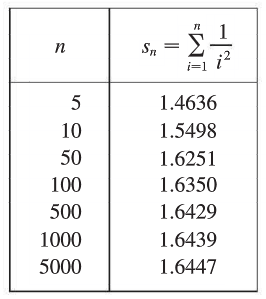
\includegraphics[scale=0.45]{11-3pic1.png}\]

We can confirm this impression with a geometric argument. The figure below shows the curve $y=\ds\frac{1}{x^2}$ and rectangles that lie below the curve. The base of each rectangle is an interval of length 1; the height is equal to the value of the function $y=\ds\frac{1}{x^2}$ at the right endpoint of the interval.

\[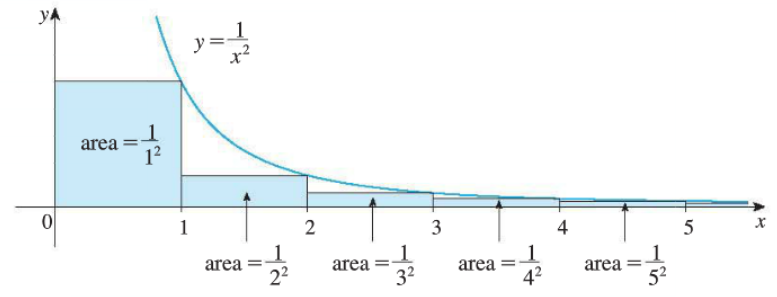
\includegraphics[scale=0.45]{11-3pic2.png}\]

So the sum of the areas of the rectangles is

\[\ds\frac{1}{1^2} + \ds\frac{1}{2^2} + \ds\frac{1}{3^2} + \ds\frac{1}{4^2} + \ds\frac{1}{5^2} + \cdots = \ds\sum_{n=1}^\infty \ds\frac{1}{n^2}\]

If we exclude the first rectangle, the total area of the remaining rectangle is smaller than the area under the curve $y=\ds\frac{1}{x^2}$ for $x\geq 1$, which is the value of the integral $\ds\int_{1}^\infty \ds\frac{1}{x^2}\text{ }dx$. In Section 7.8 we discovered that this improper integral is convergent and has value 1. So the picture shows that all the partial sums are less than

\[1+\ds\int_1^\infty \ds\frac{1}{x^2}\text{ } dx = 2.\]

Thus the partial sums are \underline{\hspace{1.25in}}. We also know that the partial sums are \underline{\hspace{1.25in}} (because all the terms are positive). Therefore the partial sums \underline{\hspace{1.25in}} (by the Monotonic Sequence Theorem) and so the series is \underline{\hspace{1.25in}}. The sum of the series (the limit of the partial sums) is then also less than 2:

\[\ds\sum_{n=1}^\infty \ds\frac{1}{n^2} < 2.\]

\underline{Fun Fact}: The exact sum of this series was found by Swiss mathematician Leonhard Euler to $\ds\frac{\pi^2}{6}$.\\
\indent

Next consider the series:
\[\ds\sum_{n=1}^\infty \ds\frac{1}{\sqrt{n}} = \ds\frac{1}{\sqrt{1}} + \ds\frac{1}{\sqrt{2}} + \ds\frac{1}{\sqrt{3}} + \ds\frac{1}{\sqrt{4}} + \ds\frac{1}{\sqrt{5}} + \cdots \]

\[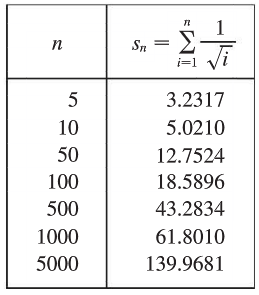
\includegraphics[scale=0.45]{11-3pic4.png}\]

The table of values of $S_n$ suggests that the partial sums aren't approaching a finite number, so we suspect that the given series may be \underline{\hspace{1.25in}}. Again we use a picture for confirmation. The figure below shows the curve $y=\ds\frac{1}{\sqrt{x}}$, but this time we use rectangles whose tops lie \textit{above} the curve.

\[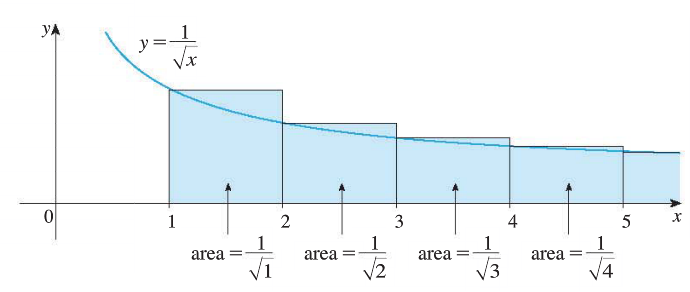
\includegraphics[scale=0.45]{11-3pic3.png}\]

The base of each rectangle is an interval of length 1. The height is equal to the value of the function $y=\ds\frac{1}{\sqrt{x}}$ at the \textit{left} endpoint of the interval. So the sum of the areas of all the rectangles is:

\[\ds\frac{1}{\sqrt{1}} + \ds\frac{1}{\sqrt{2}} + \ds\frac{1}{\sqrt{3}} + \ds\frac{1}{\sqrt{4}} + \ds\frac{1}{\sqrt{5}} + \cdots  = \ds\sum_{n=1}^\infty \ds\frac{1}{\sqrt{n}}\]\\
\indent\\
\indent

This total area is greater than the area under the curve $y=\ds\frac{1}{\sqrt{x}}$ for $x\geq 1$, which is equal to the value of the integral, $\ds\int_1^\infty \ds\frac{1}{\sqrt{x}}\text{ }dx$. But we know from Section 7.8 that this improper integral is \underline{\hspace{1.25in}} ($p=\ds\frac{1}{2} < 1$). In other words, the area under the curve is infinite. So the sum of\\
\indent\\
 the series must be \underline{\hspace{1in}}; that is, the series is \underline{\hspace{1.15in}}.\\
\indent\\
\indent

The same sort of geometric reasoning that we used for these two series can be used to prove the following test. (proof omitted )\\
\indent


\fbox{
  \parbox{\textwidth}{
  \vspace{5pt} \textbf{\underline{The Integral Test}}: \\
  \indent
  
  Suppose $f$ is a \underline{\hspace{1.25in}}, \underline{\hspace{1.25in}}, \underline{\hspace{1.25in}} function on $[1,\infty)$ and let $a_n = f(n)$. Then the series $\ds\sum_{n=1}^\infty a_n$ is convergent if and only if the improper integral $\ds\int_1^\infty f(x)\text{ }dx$ is convergent. In other words:
  \begin{enumerate}
  \item[(i)] If $\ds\int_1^\infty f(x)dx$ is \underline{\hspace{1.25in}}, then $\ds\sum_{n=1}^\infty a_n$ is \underline{\hspace{1.25in}}.\\
  \item[(ii)] If $\ds\int_1^\infty f(x)\text{ }dx$ is \underline{\hspace{1.25in}}, then $\ds\sum_{n=1}^\infty a_n$ is \underline{\hspace{1.25in}}.\\
  \end{enumerate}
  }}
  \indent\\
  \indent
  
  \underline{NOTE 1}: When we use the Integral Test, it is NOT necessary to start the series or the integral at $n=1$. For instance, in testing the series
  
  \[\ds\sum_{n=4}^\infty \ds\frac{1}{(n-3)^2} \quad \text{ we use } \quad \ds\int_4^\infty \ds\frac{1}{(x-3)^2}\text{ }dx.\]
  
  Also it is not necessary that $f$ be always decreasing. What is important is that $f$ be \textit{ultimately} decreasing, that is, decreasing for $x$ larger than some number $N$. Then $\ds\sum_{n=N}^\infty a_n$ is convergent, so $\ds\sum_{n=1}^\infty a_n$ is convergent (by Note 4 of Section 11.2).\\
  \indent
  
  
  \underline{Example 1}: Test the series $\ds\sum_{n=1}^\infty \ds\frac{1}{n^2+1}$ for convergence or divergence.\\
  \indent
  
  \textbf{SOLUTION}:\\
  \indent
  
  \vspace{4in}
  
  \underline{Example 2}: For what values of $p$ is the series $\ds\sum_{n=1}^\infty \ds\frac{1}{n^p}$ convergent?\\
  \indent
  
  \textbf{SOLUTION}: \\
  \indent
  
  If $p<0$, then $\ds\lim_{n\to\infty}\ds\frac{1}{n^p} = \underline{\hspace{0.3in}}$. If $p=0$, then $\ds\lim_{n\to\infty}\ds\frac{1}{n^p} = \underline{\hspace{0.3in}}$. In either case, $\ds\lim_{n\to\infty}\ds\frac{1}{n^p}\neq 0$, so the given series \underline{\hspace{1in}} by the Test for Divergence.\\
  \indent
  
  If $p>0$, then the function $f(x)=\ds\frac{1}{x^p}$ is clearly continuous, positive, and decreasing on $[1,\infty)$. We found in Chapter 7 that
  
  \[\ds\int_1^\infty \ds\frac{1}{x^p}\text{ }dx \text{ \underline{\hspace{1in}}  if } p>1 \text{ and \underline{\hspace{1in}}  if } p\leq 1.\]
  \indent
  
  It then follows from the Integral Test that the series $\ds\sum \ds\frac{1}{n^p}\ldots$
  \begin{itemize}
  \item \underline{\hspace{1in}}  if $p>1$\\
  \item \underline{\hspace{1in}}  if  $0<p\leq 1$
  \end{itemize}
  
  For $p=1$, this series is the \underline{\hspace{1.25in}} \underline{\hspace{1in}} , $\ds\sum_{n=1}^\infty \ds\frac{1}{n}$.\\
  \indent
  
  The series $\ds\sum_{n=1}^\infty \ds\frac{1}{n^p}$ is called the \underline{\hspace{1.25in}}. To summarize,\\
  \indent\\
  
\fbox{
  \parbox{\textwidth}{
  \vspace{5pt} \[\text{The $p-$series $\ds\sum_{n\to\infty}\ds\frac{1}{n^p}$ is convergent if $p>1$ and divergent if $p\leq 1$.}\]}}
  \indent\\
 
  
  \underline{Example 3}:
  \vspace{-10pt}
  \begin{enumerate}
  \item[(a)] The series $\ds\sum_{n=1}^\infty \ds\frac{1}{n^3}$ is \underline{\hspace{1.25in}} because it is a $p-$series with $p=3>1$.\\
  \text{ }\\
  \item[(b)] The series $\ds\sum_{n=1}^\infty \ds\frac{1}{n^{1/3}}$ is \underline{\hspace{1.25in}} because it is a $p-$series with $p=\ds\frac{1}{3}<1$.\\
  \end{enumerate}
  \indent\\
  \indent
  
  \underline{NOTE 2}: We should NOT infer from the Integral Test that the sum of the series is \underline{\hspace{1in}}  to the value of the integral. In fact, 
  
  \[\ds\sum_{n=1}^\infty \ds\frac{1}{n^2} = \underline{\hspace{0.5in}} \quad \text{ whereas } \quad \ds\int_1^\infty \ds\frac{1}{x^2}dx = \underline{\hspace{0.5in}}.\]
  \indent
  
  Therefore, in general,
  \vspace{-10pt}
  \[\ds\sum_{n=1}^\infty a_n\neq \ds\int_1^\infty f(x)\text{ }dx.\]
  
  
  
\underline{Example 4}: Determine whether the series $\ds\sum_{n=1}^\infty \ds\frac{\ln n}{n}$ converges of diverges.\\
\indent

\textbf{SOLUTION}: The function $f(x)=\ds\frac{\ln x}{x}$ is positive and continuous for $x>1$ because the logarithm function is continuous. But it is not obvious whether or not $f$ is decreasing, so we compute its derivative:

\[f'(x) = \hspace{3.5in}\]

\indent

Thus $f'(x)<0$ when $\ln x>1 \implies \underline{\hspace{1in}}$. It follows that $f$ is decreasing when $x>e$ and so we can apply the \underline{\hspace{1in}} \underline{\hspace{1in}}:\\
\indent

\vspace{2in}

Since this improper integral is \underline{\hspace{1.25in}}, the series $\ds\sum_{n=1}^\infty \ds\frac{\ln n}{n}$ is also \underline{\hspace{1.25in}} by the Integral Test.


\section*{Estimating the Sum of a Series}
Suppose we have been able to use the Integral Test to show that a series $\ds\sum a_n$ is convergent and now we want to find an approximation to the sum $S$ of the series. Of course, any partial sum $S_n$ is an approximation to $S$ because $\ds\lim_{n\to\infty}S_n=S$. But how good is such an approximation? To find out, we need to estimate the size of the \underline{\hspace{1.25in}}

\[R_n = \underline{\hspace{1in}} = a_{n+1} + a_{n+2} + a_{n+3} + \cdots\]
\indent

The remainder $R_n$ is the \underline{\hspace{1in}} made when $S_n$, the sum of the first $n$ terms, is used as an approximation to the total sum.

\[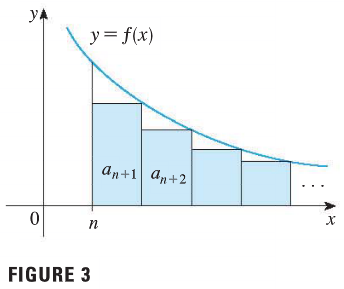
\includegraphics[scale=0.5]{11-3pic5.png}\quad \quad \quad 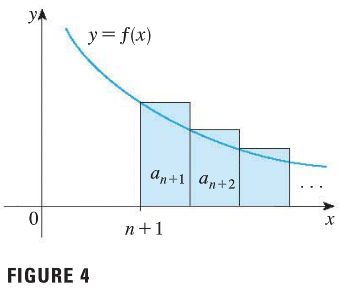
\includegraphics[scale=0.5]{11-3pic6.png}\]

We use the same notation and ideas as in the Integral Test, assuming that $f$ is decreasing on $[n,\infty)$. Comparing the areas of the rectangles with the area under $y=f(x)$ for $x>n$ in Figure 3, we see that

\[R_n = a_{n+1} + a_{n+2} + \cdots \leq \ds\int_n^\infty f(x) \text{ }dx\]

Similarly, we see from Figure 4 that

\[R_n = a_{n+1} + a_{n+2} + \cdots \geq \ds\int_{n+1}^\infty f(x)\text{ }dx\]

So we have proved the following error estimate.\\
\indent\\


\fbox{
  \parbox{\textwidth}{
  \vspace{5pt} \textbf{\underline{Remainder Estimate for the Integral Test}}: Suppose $f(k)=a_k$, where $f$ is a continuous, positive, decreasing function for $x\geq n$ and $\ds\sum a_n$ is convergent. If $R_n = S-S_n$, then
  
  \[\ds\int_{n+1}^\infty f(x) \text{ } dx \leq R_n \leq \ds\int_n^\infty f(x)\text{ }dx.\]
  
  }}
  \indent\\
  \indent
  
  \newpage
  \underline{Example 5}:
  \begin{enumerate}
  \item[(a)] Approximate the sum of the series $\ds\sum \ds\frac{1}{n^3}$ by using the sum of the first 10 terms. Estimate the error involved in this approximation.
  \item[(b)] How many terms are required to ensure that the sum is accurate to within 0.0005?
  \end{enumerate}
  \indent
  
  \textbf{SOLUTION}: 
  
  
  \newpage
  
  If we add $S_n$ to each side of the inequalities in the Remainder Estimate for the Integral Test, we get\\
  \indent
  
  \fbox{
  \parbox{\textwidth}{
  \vspace{5pt} 
  \[S_n + \ds\int_{n+1}^\infty f(x)\text{ }dx \leq S \leq S_n + \ds\int_n^\infty f(x)\text{ }dx \hspace{1.5in} (3)\]
  }}
  \indent\\
  \indent
  
  because $S_n + R  = S$. These inequalities $(3)$ give a lower bound and an upper bound for $S$, the sum of the series. They provide a more accurate (or tighter) approximation to the sum of the series than the partial sum $S_n$ alone does.\\
  \indent
  
  \underline{Example 6}: Use inequalities $(3)$ with $n=10$ to estimate the sum of the series $\ds\sum_{n=1}^\infty \ds\frac{1}{n^3}$.\\
  \indent
  
  \textbf{SOLUTION}: \\
  \indent
  
  \vspace{4in}
  
  If we approximate $S$ by the midpoint of this interval, then the error is at most half the length of the interval. So
  
  \[\ds\sum_{n=1}^\infty \ds\frac{1}{n^3} \approx \underline{\hspace{1.25in}} \quad \text{ with error } < \underline{\hspace{1.25in}}\]
  \indent
  
  \underline{NOTE}: If we compare Example 6 with Example 5, we see the improved estimate using inequalities $(3)$ can be much better than the estimate $S\approx S_n$. To make the error smaller than 0.0005 we had to use 32 terms in Example 5 but only 10 terms in Example 6.\\
  \indent
  

%----------------------------------------------------------------------------------------

\end{document}